% Source-derived anatomy visualization; no generated biology or pixel edits.
\documentclass[tikz,border=2pt]{standalone}
\usepackage[T1]{fontenc}
\usepackage{graphicx}
\usepackage{xcolor}
\usetikzlibrary{arrows.meta}

\definecolor{ink}{HTML}{233747}
\definecolor{blue}{HTML}{256B91}
\definecolor{bluebg}{HTML}{EAF2F7}
\definecolor{orange}{HTML}{B95020}
\definecolor{grey}{HTML}{68747D}

\begin{document}
\begin{tikzpicture}[
  x=1cm,y=1cm,
  every node/.style={font=\sffamily\fontsize{8}{9.5}\selectfont,text=ink,align=center},
  heading/.style={font=\sffamily\bfseries\fontsize{11}{13}\selectfont},
  panel heading/.style={font=\sffamily\bfseries\fontsize{9}{11}\selectfont,text=blue},
  label/.style={font=\sffamily\bfseries\fontsize{8}{9.5}\selectfont,fill=white,fill opacity=.88,text opacity=1,inner sep=2pt,rounded corners=1pt},
  arrow/.style={-{Stealth[length=4pt]},line width=.8pt,draw=orange}
]

\path[use as bounding box] (0,0) rectangle (16.8,8.6);
\node[heading,anchor=west,text=orange] at (.1,8.28) {Fly brain and ventral nerve cord};

\draw[draw=blue!35,fill=bluebg!45,rounded corners=4pt,line width=.65pt]
  (0,.55) rectangle (7.55,7.85);
\draw[draw=blue!35,fill=bluebg!45,rounded corners=4pt,line width=.65pt]
  (7.85,.55) rectangle (16.8,7.85);

\node[panel heading] at (3.78,7.48) {Frontal view};
\node at (2.85,4.10)
  {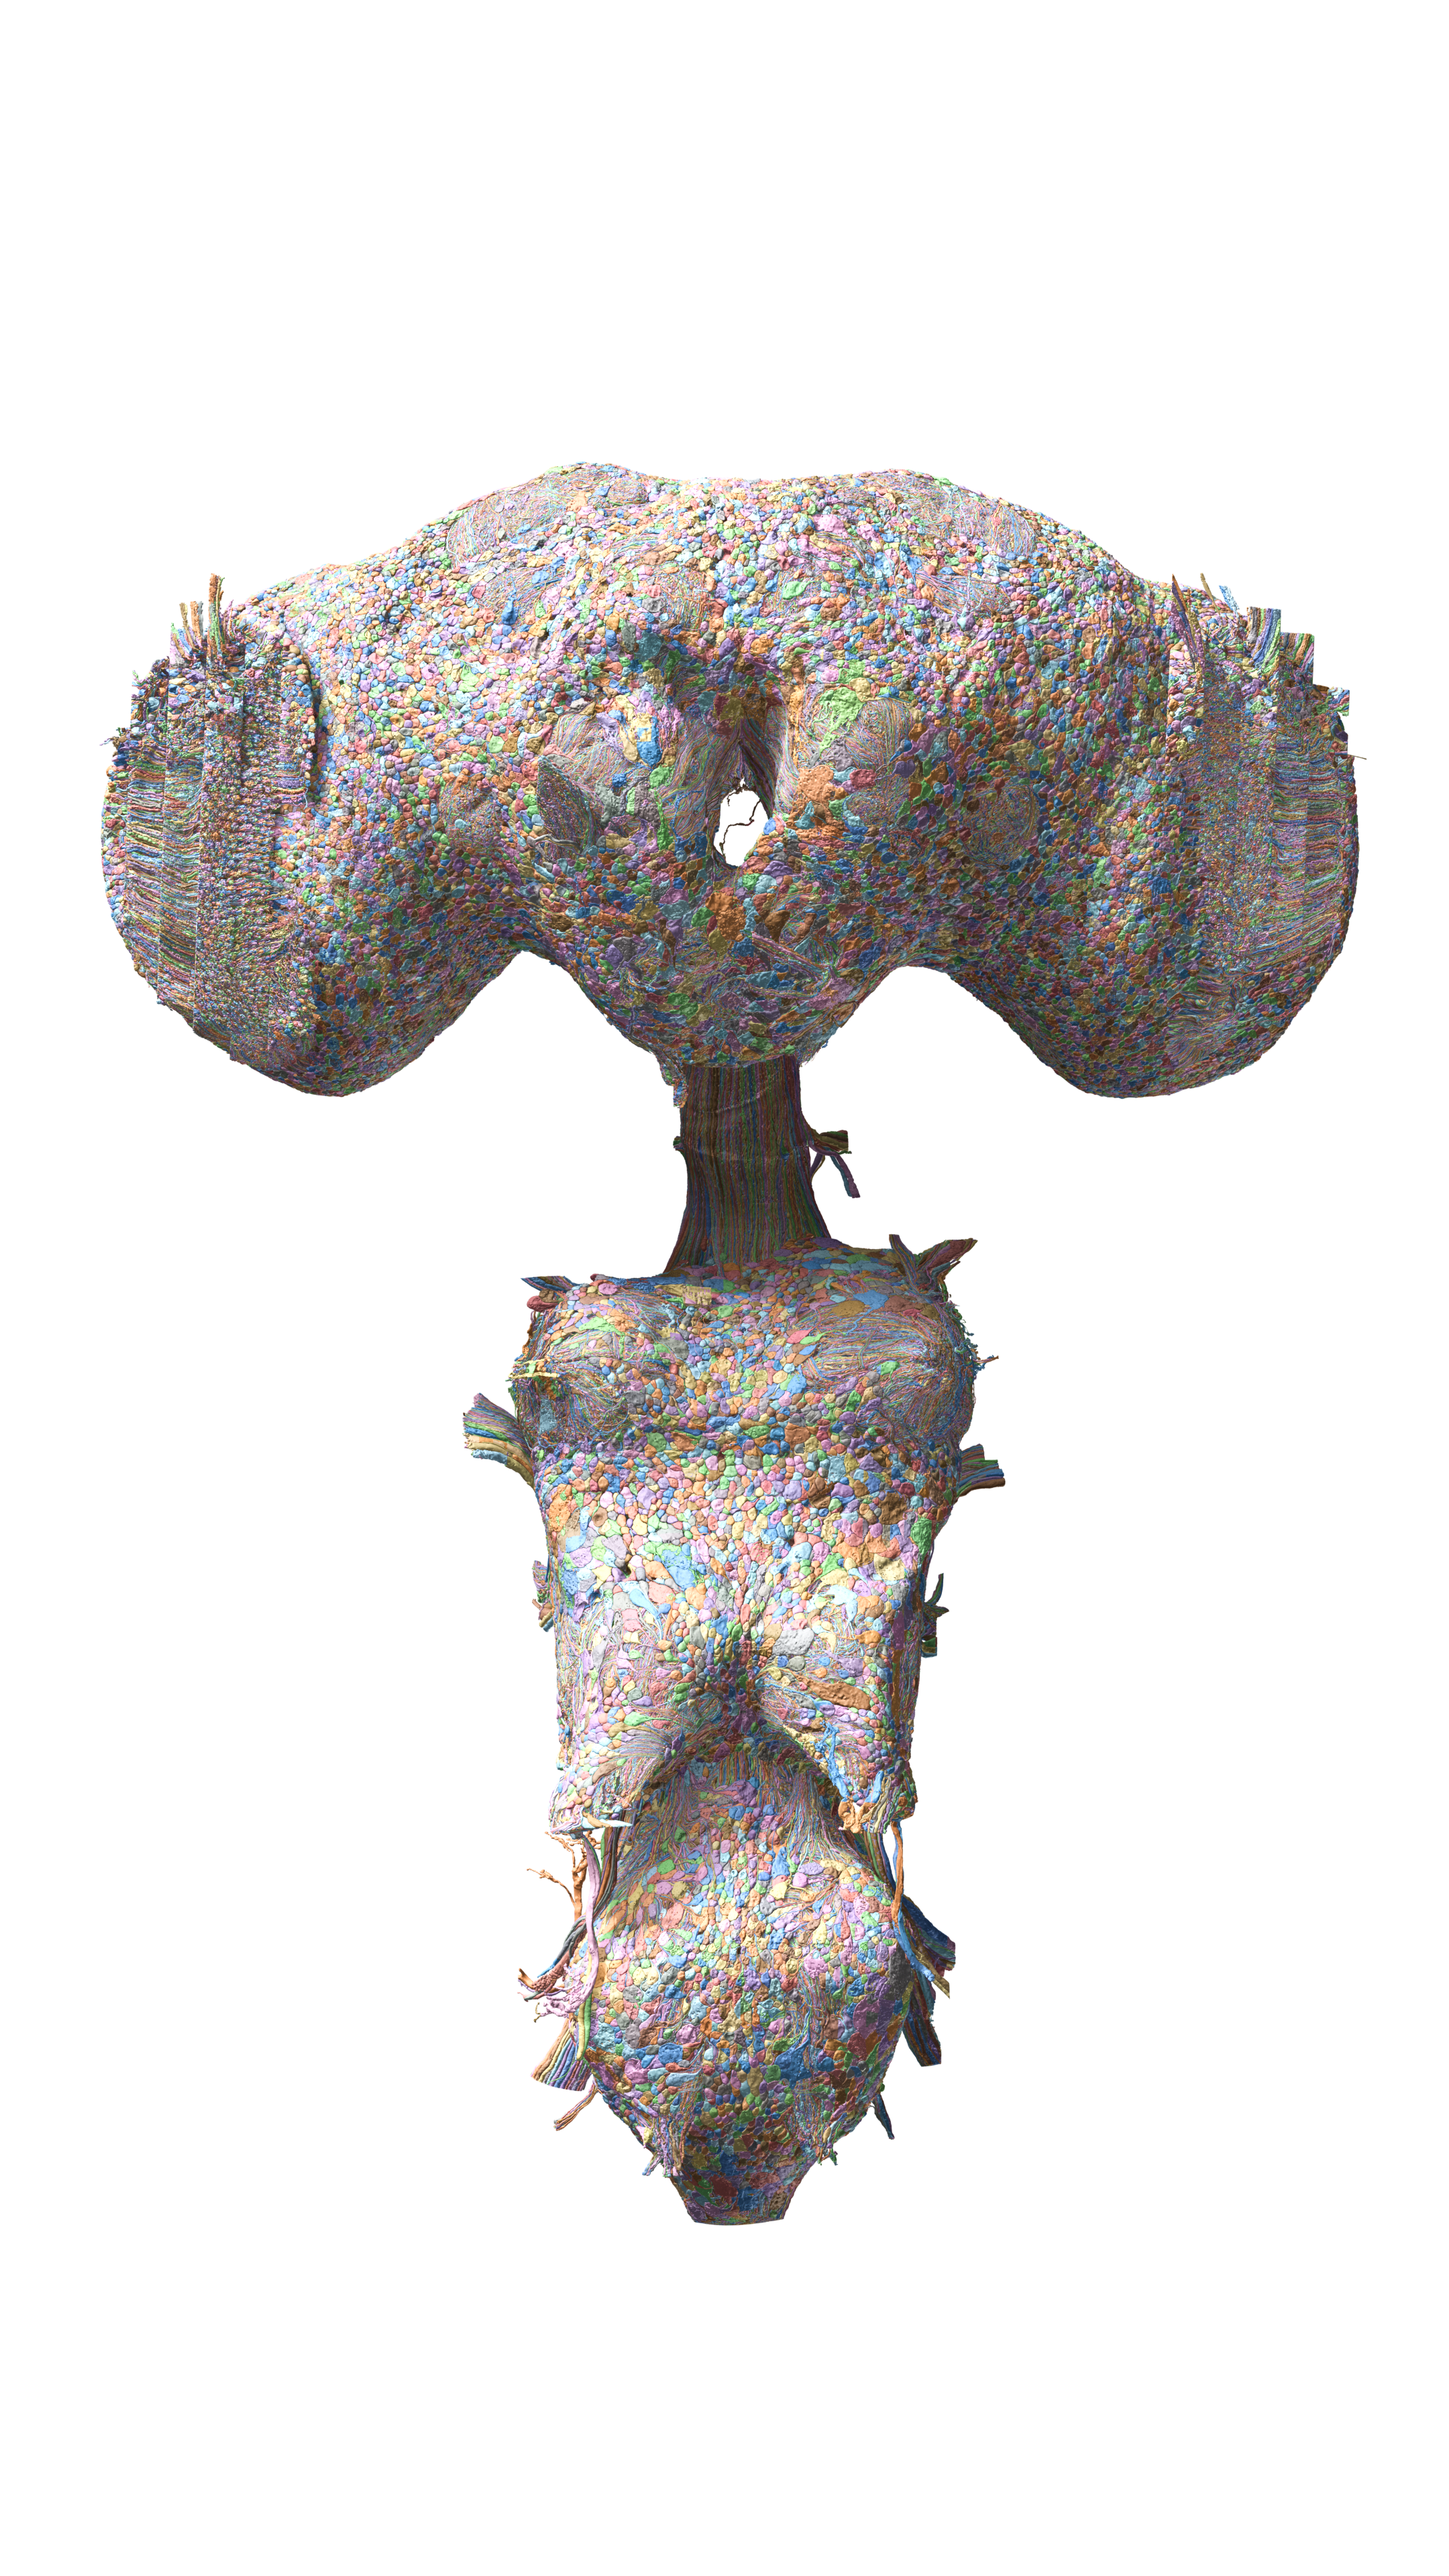
\includegraphics[height=6.25cm,trim=120 470 100 640,clip]{fly_brain_vnc.png}};
\node[label,anchor=west] (brain) at (5.10,6.38) {brain};
\draw[arrow] (brain.west) -- (4.02,6.25);
\node[label,anchor=west,text=orange] (vnc) at (4.92,3.05) {VNC};
\draw[arrow] (vnc.west) -- (3.70,3.12);
\node[font=\sffamily\fontsize{7}{8.5}\selectfont,text=grey] at (3.78,.90)
  {MaleCNS source rendering};

\node[panel heading] at (12.33,7.48) {Lateral context};
\node at (12.33,4.35)
  {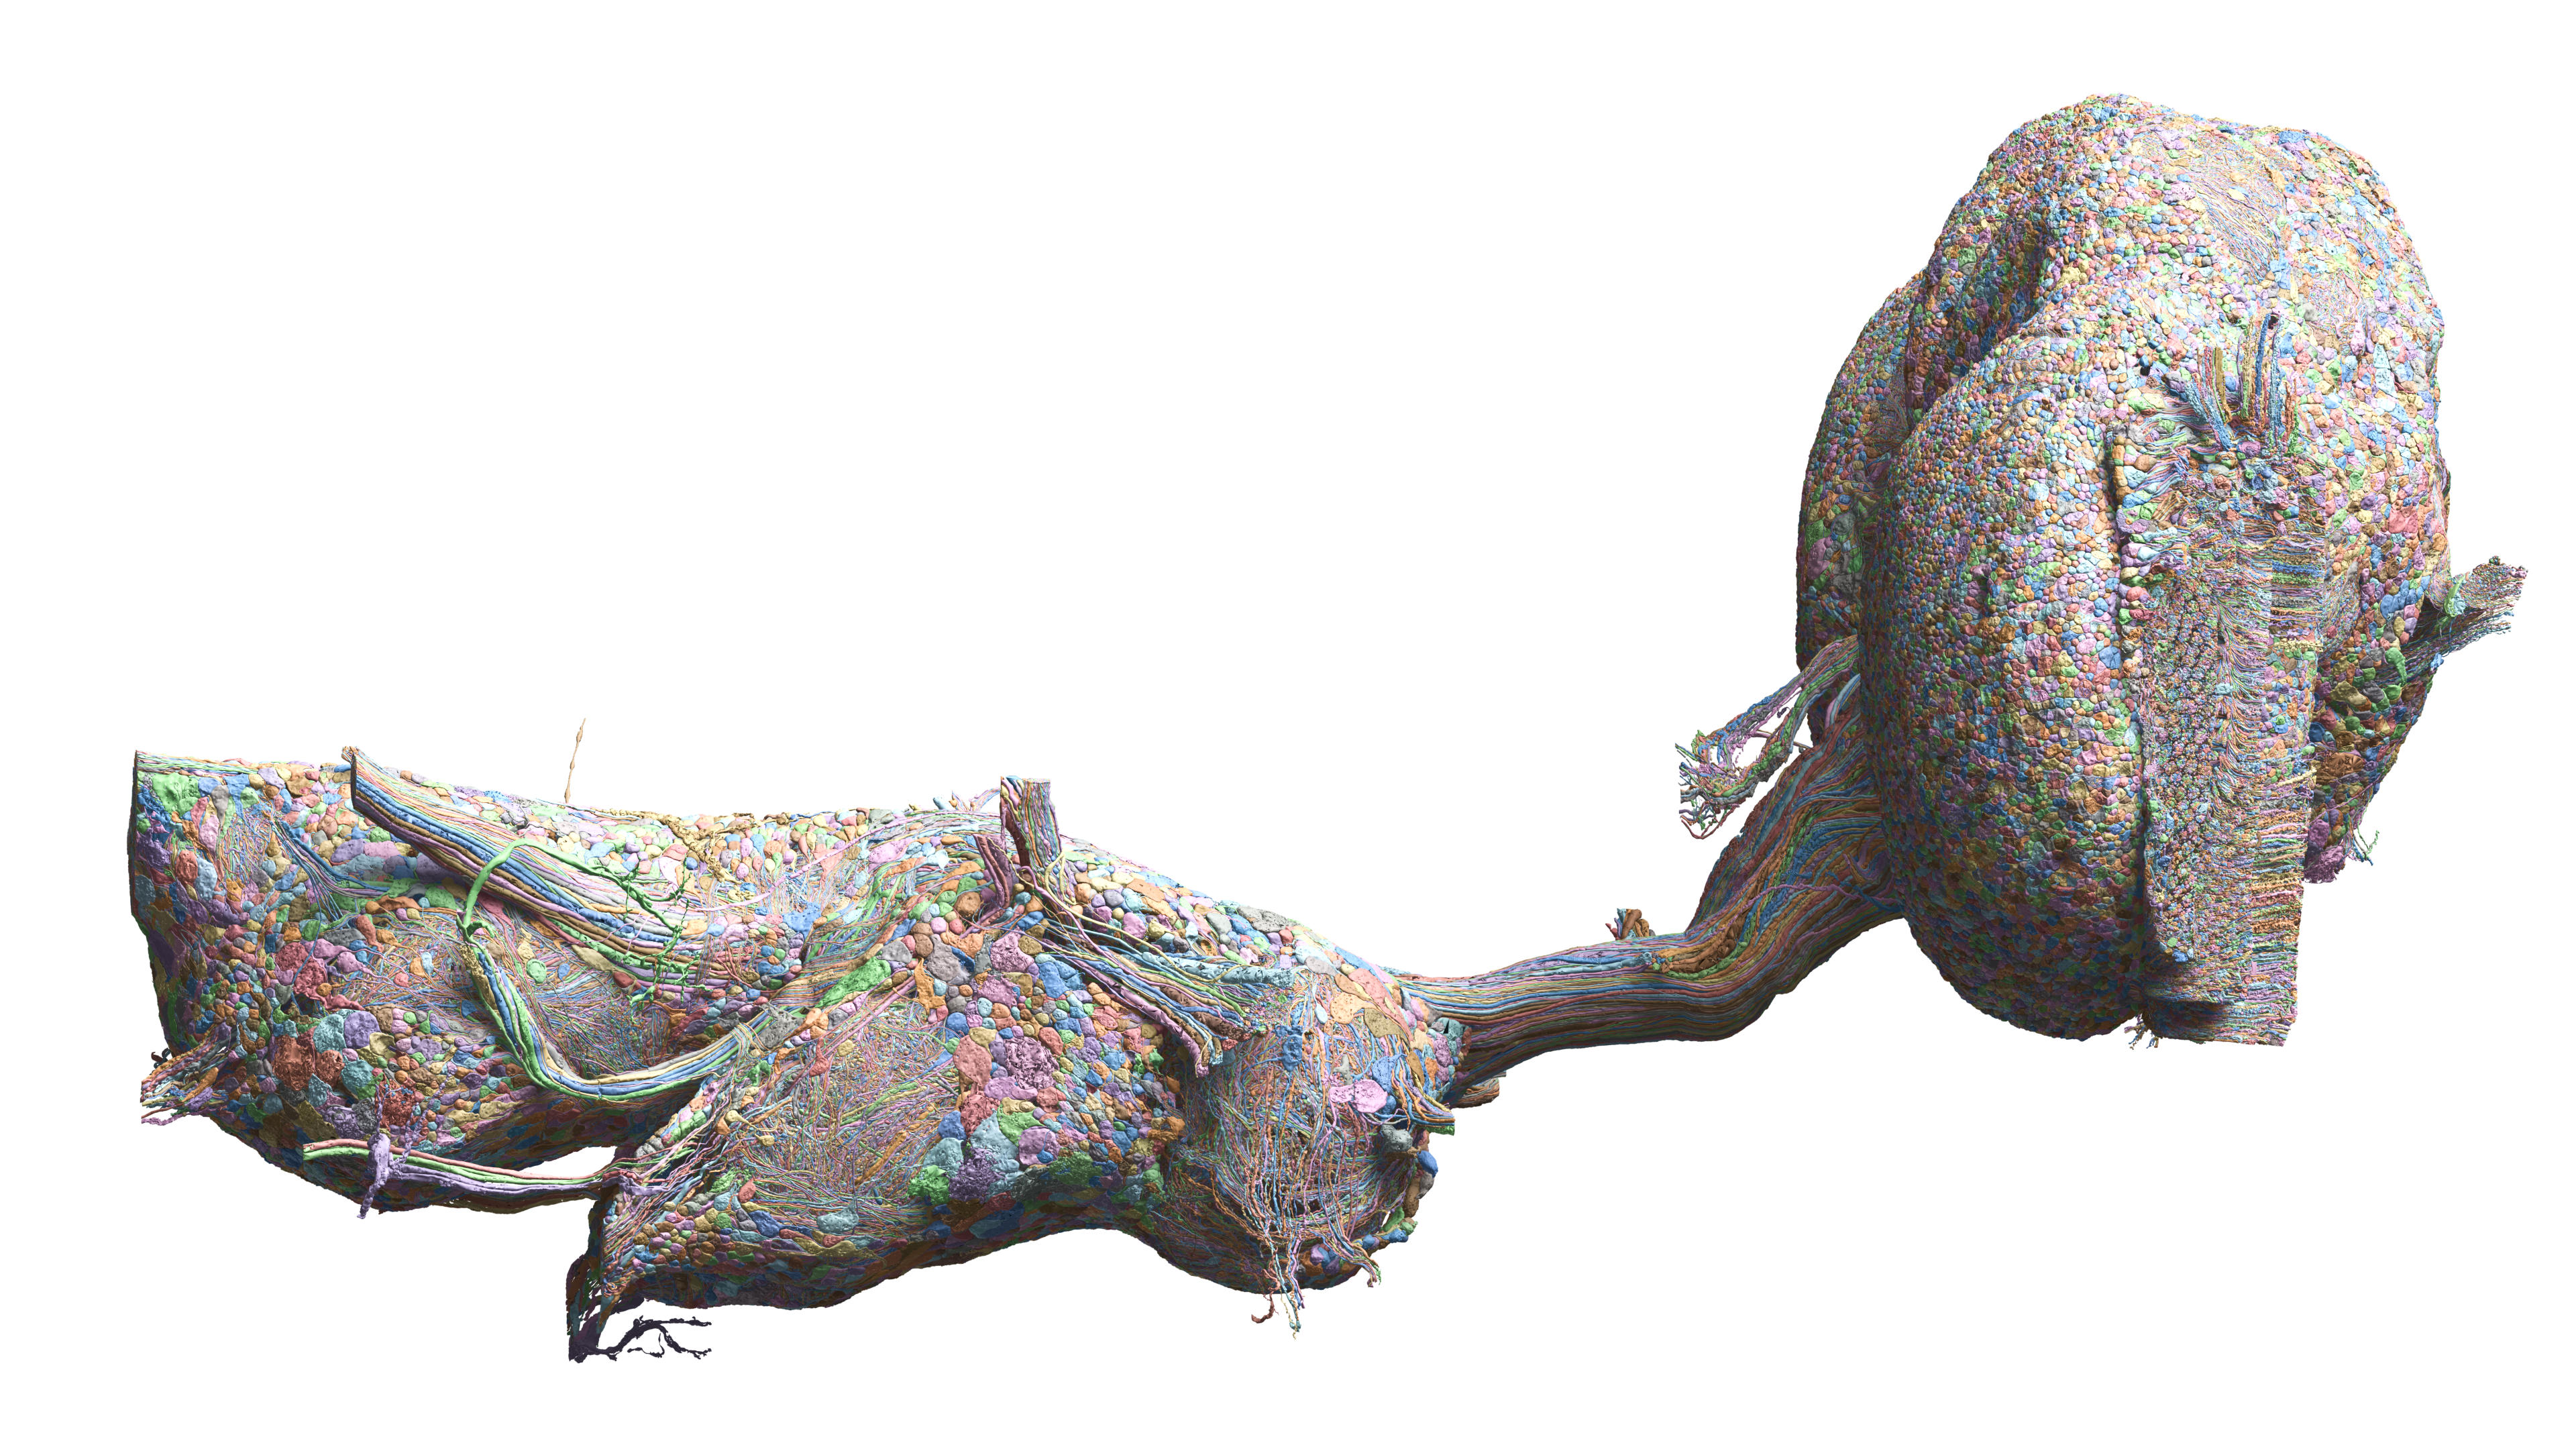
\includegraphics[width=8.25cm,height=4.75cm,keepaspectratio]{fly_cns_lateral.png}};
\node[label,anchor=west] (brainlat) at (14.78,6.04) {brain};
\draw[arrow] (brainlat.west) -- (14.02,5.75);
\node[label,anchor=east,text=orange] (vnclat) at (9.10,2.35) {VNC};
\draw[arrow] (vnclat.east) -- (10.15,3.20);
\node[font=\sffamily\fontsize{7}{8.5}\selectfont,text=grey] at (12.33,.90)
  {Orientation follows source visualization; no anatomical scale asserted};

\end{tikzpicture}
\end{document}
